\chapter{Theory}

\section{Furuta's Pendulum}

Rotational inverted pendulum or Furuta’s pendulum composes of two main parts: motor-driven arm, which rotates in the horizontal plane and a pendulum, attached to that arm, which freely rotates in the vertical plane. The system is underactuated and extremely nonlinear due to the gravitational forces and the coupling arising from the Coriolis and centripetal forces. The schematic representation of the pendulum is shown in \ref{furuta}
\begin{figure}[h]
	\centering
	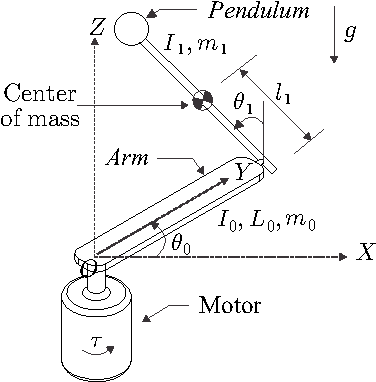
\includegraphics[width=.6\linewidth]{images/furuta}
	\caption{Furuta's Pendulum}
	\label{furuta}
\end{figure}
\newpage
The symbols in the figure indicate the following:
\begin{itemize}
	\item \textbf{$g$} - gravitational acceleration [\si{\metre\per\square\second}]
	\item \textbf{$m_0$} - mass of arm [\si{\kilogram}]
	\item \textbf{$m_1$} - mass of pendulum [\si{\kilogram}]
	\item \textbf{$L_0$} - length of arm [\si{\metre}]
	\item \textbf{$L_1$} - length of pendulum [\si{\metre}]
	\item \textbf{$l_1$} - location of the pendulums center of mass [\si{\metre}]
	\item \textbf{$I_0$} - moment of inertia of arm [\si{\kilogram\per\square\metre}]
	\item \textbf{$I_1$} - moment of inertia of pendulum [\si{\kilogram\per\square\metre}]
	\item \textbf{$\theta_0$} - arm angle [\si{\radian}]
	\item \textbf{$\theta_1$} - pendulum angle [\si{\radian}]
	\item \textbf{$\tau$} - motor torque [\si{\volt}]
\end{itemize}
\subsection{State-Space Representation}
To obtain the state representation of the process we must define our state variables first:
\begin{equation}
	\begin{bmatrix}
	x_1 & x_2 & x_3 & x_4
	\end{bmatrix}^\intercal = 
	\begin{bmatrix}
	\theta_0 & \dot{\theta_0} & \theta_1 & \dot{\theta_1}
	\end{bmatrix}^\intercal
\end{equation}
Control variable:
\begin{equation} u = \tau \end{equation}
Then we can write our state equations:
\begin{subequations}
\begin{equation}\dot{x_1} = \dot{\theta_0} \end{equation}
\begin{equation}\dot{x_2} = \frac{\gamma(\epsilon\dot{\theta_0}^2+\rho)-\delta(\tau+\beta\dot{\theta_1}^2-\sigma\dot{\theta_0}\dot{\theta_1})}{\gamma^2-\alpha\delta}\end{equation}
\begin{equation}\dot{x_3} = \dot{\theta_1}\end{equation}
\begin{equation}\dot{x_4} = \frac{\gamma(\tau+\beta\dot{\theta_1}^2-\sigma\dot{\theta_0}\dot{\theta_1})-\alpha(\epsilon\dot{\theta_0}^2+\rho)}{\gamma^2-\alpha\delta}\end{equation}
\end{subequations}
where
\begin{equation}\alpha = I_0+L_0^2m_1+l_1^2m_1\sin^2\theta_1\end{equation}
\begin{equation}\beta = L_0m_1l_1\sin\theta_1 \end{equation}
\begin{equation}\gamma = L_0m_1l_1\cos\theta_1\end{equation}
\begin{equation}\delta = I_1+l_1^2m_1\end{equation}
\begin{equation}\epsilon = l^2_1m_1\sin\theta_1\cos\theta_1\end{equation}
\begin{equation}\rho = m_1gl_1\sin\theta_1\end{equation}
\begin{equation}\tau = 2l^2_1m_1\sin\theta_1\cos\theta_1\end{equation}
Now these non-linear differential equations we can write in the form of matrices:
\begin{equation}\label{nonlinmodel}
\begin{bmatrix}
\dot{x_1} \\ \dot{x_2} \\ \dot{x_3} \\ \dot{x_4}
\end{bmatrix} = \begin{bmatrix}
\dot{\theta_0}\\
\frac{\gamma(\epsilon\dot{\theta_0}^2+\rho)-\delta(\tau+\beta\dot{\theta_1}^2-\sigma\dot{\theta_0}\dot{\theta_1})}{\gamma^2-\alpha\delta}\\
\dot{\theta_1}\\
 \frac{\gamma(\tau+\beta\dot{\theta_1}^2-\sigma\dot{\theta_0}\dot{\theta_1})-\alpha(\epsilon\dot{\theta_0}^2+\rho)}{\gamma^2-\alpha\delta}
\end{bmatrix}
\end{equation}
or:
\begin{equation}\dot{\textbf{x}} = f(\textbf{x},u) =\begin{bmatrix}f_1(\textbf{x},u)\\f_2(x,u)\\f_3(x,u)\\f_4(x,u)\end{bmatrix} \end{equation}
So that’s our non-linear dynamic model of the process. But only the NMPC controller is able to operate with such a model.  So, to make that model suitable for LQR and MPC controller we can approximate that non-linear model by a linear model as follows:
\begin{equation}\dot{x} = Ax + Bu\end{equation}
And the constant matrices are derived as:
\begin{equation}
A = \begin{bmatrix}
\frac{\partial f_1(x,u)}{\partial x_1}&\frac{\partial f_1(x,u)}{\partial x_2}&\frac{\partial f_1(x,u)}{\partial x_3}&\frac{\partial f_1(x,u)}{\partial x_4}\\
\frac{\partial f_2(x,u)}{\partial x_1}&\frac{\partial f_2(x,u)}{\partial x_2}&\frac{\partial f_2(x,u)}{\partial x_3}&\frac{\partial f_2(x,u)}{\partial x_4}\\
\frac{\partial f_3(x,u)}{\partial x_1}&\frac{\partial f_3(x,u)}{\partial x_2}&\frac{\partial f_3(x,u)}{\partial x_3}&\frac{\partial f_3(x,u)}{\partial x_4}\\
\frac{\partial f_4(x,u)}{\partial x_1}&\frac{\partial f_4(x,u)}{\partial x_2}&\frac{\partial f_4(x,u)}{\partial x_3}&\frac{\partial f_4(x,u)}{\partial x_4}
\end{bmatrix}
\end{equation}
respektive:
\begin{equation}
	A =\begin{bmatrix}0&1&0&0\\
	0&0&\frac{-gL_0l_1^2m_1^2}{(m_1L_0^2+I_0)(m_1l_1^2+I_1)-L_0^2l_1^2m_1^2}&0\\
	0&0&0&1\\
	0&0&\frac{gl_1m_1(m_1L_0^2+I_0)}{(m_1L_0^2+I_0)(m_1l_1^2+I_1)-L_0^2l_1^2m_1^2}&0
	\end{bmatrix}
\end{equation}
\begin{equation}B = \begin{bmatrix}
\frac{\partial f_1(x,u)}{\partial u}\\\frac{\partial f_2(x,u)}{\partial u}\\\frac{\partial f_3(x,u)}{\partial u}\\\frac{\partial f_4(x,u)}{\partial u}
\end{bmatrix}=\begin{bmatrix}
0\\ 
\frac{m_1L_1^2+I_1}{(m_1L_0^2+I_0)(m_1l_1^2+I_1)-L_0^2l_1^2m_1^2}\\0\\
\frac{-L_0l_1m_1}{(m_1L_0^2+I_0)(m_1l_1^2+I_1)-L_0^2l_1^2m_1^2}
\end{bmatrix}\end{equation}
\begin{equation}C = \begin{bmatrix}0&0&1&0\end{bmatrix}\end{equation}
\begin{equation}D = 0\end{equation}
The linearized equations of motion for the simplified system are now could be derived for two equilibrium positions: upright and downward. The reason is that at the downward position the system's output, which is the position of the pendulum, has a stable point at “$+\pi$” and “$-\pi$”, while at the upright position system has no stable point.\\

The model, obtained by linearization around the upright operation point, is used for fulfilling the main control objective, which is stabilizing the pendulum at the upright position. The second model is used to simulate process behavior during initial excitation by a Swing-up controller.
\section{Controller Synthesis}
\subsection{LQR design}
The Linear Quadratic Regulator (LQR) is a well-known method that provides optimally controlled feedback gains to enable the closed-loop stable and high performance design of systems.
\begin{equation}
\begin{split}
\dot{x} &= Ax + Bu\\
y &= Cx, C=I^{n \times n}
\end{split}
\end{equation}
which requires  full-state feedback (all n states are measurable).
The feedback gain is a matrix K and the feedback control law takes the form:
\begin{equation}
	u = -Kx
\end{equation}
Than closed-loop system dynamics can be written:
\begin{equation}
\dot{x} = (A-BK)x
\end{equation}
So there appears condition that poles of $(A-BK)$ must be in in stable, suitably-damped locations in the complex plane.
\subsubsection{Derivation of LQR}
Towards a generic procedure for solving optimal control problems, we derive a methodology based on the calculus of variations. The problem statement for a fixed final time $t_f$ is:
\begin{equation}
\begin{split}
	J = \min_{u}& \quad \Phi(t_f)+\frac{1}{2}\int\limits_{t_0}^{t_f}L(x(t),u(t),t)\;dt\\
	s.t.&\quad  \dot{x} = f(x(t),u(t),t)\\
	& \quad x(t_0) = x_0
	\end{split}
\end{equation}
In the case of the Linear Quadratic Regulator (with zero terminal cost), we set  $\Phi(x(t_f))=0$, and $L = x^\intercal Qx+u^\intercal Ru$ solve the new optimization problem
\begin{equation}
J=\min_{u}  \frac{1}{2}\int\limits_{t_0}^{t_f}x^\intercal Qx+u^\intercal Ru\;dt
\end{equation}
Where $Q$ and $R$ are positive semidefinite weighting matrices for states and control input respectively.
Now we define new variable $H$ as:
\begin{equation}
H = \frac{1}{2}(x\intercal Qx + u^\intercal Ru)+\lambda^\intercal(Ax + Bu)
\end{equation}

As we are looking for minimum, we apply the condition, that $\frac{\partial H(x,u,\lambda)}{\partial u}$ is equal to zero.
\begin{equation}
	\frac{\partial H(x,u,\lambda)}{\partial u} = Ru + B^\intercal\lambda = 0
\end{equation}
then:
\begin{equation}
u = -R^{-1}B^\intercal\lambda
\end{equation}
where
\begin{equation}
\lambda = Px
\end{equation}
and finally
\begin{equation}
u = -R^{-1}B^\intercal Px
\end{equation}
And that is our optimal control law for full-state feedback LQR. Matrix $P$ is calculated by solving Riccati equation in continuous time:
\begin{equation}
Q + A^\intercal P + PA - PBR^{-1}B^\intercal P = 0
\end{equation}
\subsection{MPC controller design}
MPC uses a model of the system to make predictions about the system’s future behavior. MPC solves an online optimization algorithm to find the optimal control action that drives the predicted output to the reference. MPC can handle MIMO systems that may have interactions between their inputs and outputs. It can also handle input and output constraints. MPC has preview capability; it can incorporate future reference information into the control problem to improve controller performance.
\subsubsection{MPC formulation}
MPC controller requires the model of the system in the discrete time formulation that
is used to predict systems behavior in the future:
\begin{equation}
	\begin{split}
	&x_{k+1} = Ax_k + Bu_k\\
	&y_k = Cx_k
	\end{split}
\end{equation}
State predictions: 
\begin{equation}
\begin{split}
\hat{x}_{k+1} &= Ax_k + Bu_k\\
\hat{x}_{k+2} &= A\hat{x}_{k+1} + Bu_{k+1}\\
&= A^2x_k + ABu_k + Bu_{k+1}\\
\hat{x}_{k+3} &= A\hat{x}_{k+2} + Bu_{k+2}\\
&= A^3x_k + A^2Bu_k + ABu_{k+1} + Bu_{k+2}\\
&\vdots\\
\hat{x}_{k+N} &= A^Nx_k+\sum_{j=k}^{k+N-1}A^jBu_{k+N-j-1}
\end{split}
\end{equation}
Output Predictions:
\begin{equation}
\begin{split}
\hat{y}_{k+1} &= C\hat{x}_{k+1}\\
			  &= CAx_k + CBu_k\\
\hat{y}_{k+2} &= C\hat{x}_{k+2}\\
			  &= CA^2x_k + CABu_k + CBu_{k+1}\\
			  \hat{y}_{k+2} &= C\hat{x}_{k+2}\\
			  &= CA^3x_k + CA^2Bu_k + CABu_{k+1} + CBu_{k+2}
\end{split}
\end{equation}
Now we can obtain predictive system model:
\begin{equation}
	\begin{bmatrix}
	\hat{y}_{k+1}\\\hat{y}_{k+2}\\ \vdots\\ \hat{y}_{k+N}
	\end{bmatrix} = \begin{bmatrix}CA\\CA^2\\ \vdots \\ CA^N\end{bmatrix}x_k + \begin{bmatrix}CB& 0&\cdots&0\\
	CAB&CB&\cdots&0\\
	\vdots&\vdots&\ddots&\vdots\\
	CA^{N-1}&CA^{N-2}&\cdots&CB\end{bmatrix}\begin{bmatrix}u_k\\u_{k+1}\\\vdots\\u_{k+N-1}\end{bmatrix}
\end{equation}
respektive:
\begin{equation}
	\hat{Y} = Y_0 + GU
\end{equation}
And now the whole optimization problem could be written as a QP problem with constrains:
\begin{equation}\label{mpcformulation}
\begin{split}
J = \min_{u}& \sum_{k}^{k+N}x^\intercal Q_xx+u^\intercal Q_uu\\
s.t.&\quad  x_{k+1} = Ax_k + Bu_k\\
&\quad  y_{k} = Cx_k\\
& \quad u_{min}\leq u_k\leq u_{max}
\end{split}
\end{equation}
Where $Q_x$ and $Q_u$ are positive semidefinite weighting matrices for states and control input respectively.
By solving that optimization problem we get the optimal value for control input for every simulation step.
\subsection{Swing-Up controller design}
For initial excitation of the system we use the energy-based swing-up controller. The strategy with this controller is that we increase the amplitude of swings by increasing the energy of the system with every swing. The energy is added by controlling arms movements and depends on the actual energy of the pendulum. The actual energy of the pendulum can be calculated from the actual position of the pendulum and its velocity: 
\begin{equation}
E = \frac{m_1gl_1}{2}((\frac{\dot{\theta_1}}{\omega_0})^2+\cos\theta_1 - 1)
\end{equation}
Than the control law has following form:
\begin{equation}
	u = k_vEsign(\dot{\theta_1}\cos\theta_1)
\end{equation}
Where element $sign(\dot{\theta_1}\cos\theta_1)$ determines direction i which the force will be applied and $k_vE$ is the gain of the controller.







